%%% Kapitola – Výzvy a problémy
%%%%% Wording: ⏳
%%%%% Styling: ⏳
%%%%% References: ⏳
%%% --------------------------------------------------------------
\chapter{Výzvy a problémy}
\label{ch:vyzvy-a-problemy}
Tato kapitola se zabývá hlavními výzvami, které se vyskytly během vývoje aplikace rezervačního systému.
Každá sekce popisuje konkrétní problém, který byl řešen, různé alternativy, které byly zvažovány, a konečná řešení, která byla implementována.
Sdílením těchto zkušeností lze dosáhnout hlubšího porozumění vývojového procesu a složitého rozhodování, které je zapotřebí.

%%% Sekce – Vykreslování interaktivního plánu sezení pomocí SVG
%%%%% Wording: ⏳
%%%%% Styling: ⏳
%%%%% References: ⏳
%%% --------------------------------------------------------------
\section{Vykreslování interaktivního plánu sezení pomocí SVG}
\label{sec:vyzvy-a-problemy-rendering-sedadel}
Vykreslování interaktivního plánu sezení představovalo počáteční výzvu.
To bylo způsobeno složitostí a dynamickou povahou mapy.
Byly zvažovány různé technologie, jako je inline SVG, Canvas API a Three.js.

Po důkladném zvážení byl vybrán inline SVG, protože bylo zjištěno, že je nejjednodušší a nejpohodlnější možností, i když to nemusí být nejvýkonnější možností.
Tato metoda umožnila jednoduché a přímočaré interakce s DOM, což usnadnilo vývoj interaktivní mapy sezení.

Nicméně animace a transformace SVG představovaly další problém.
SVG prvky a HTML prvky se chovají odlišně, pokud jde o jejich počáteční body, jak je znázorněno na obrázku ~\ref{fig:css-tricks-svg-transforms} níže.

\begin{figure}[H]
    \centering
    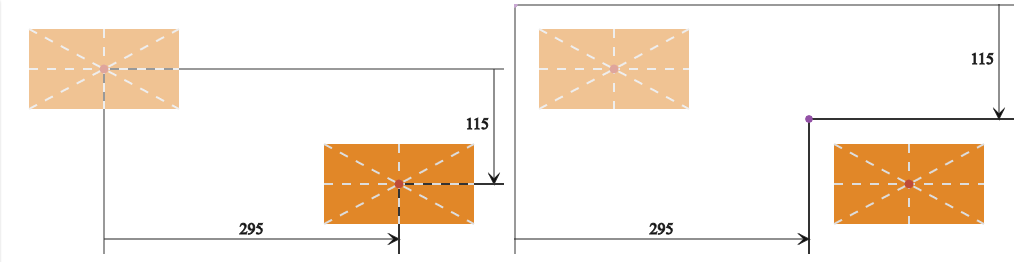
\includegraphics[0.8\textwidth]{\FIGDIR/css-tricks-svg-transforms}
    % TODO: add a reference to the image
    \caption{Počáteční body SVG a HTML}
    \label{fig:css-tricks-svg-transforms}
\end{figure}

To způsobilo neočekávané chování při implementaci určitých funkcionalit.
Nakonec bylo toto vyřešeno získáním hlubšího porozumění chování SVG a manipulací s prvky na základě tohoto chování.

%%% Sekce – Absence API a jeho simulace
%%%%% Wording: ⏳
%%%%% Styling: ⏳
%%%%% References: ⏳
%%% --------------------------------------------------------------
\section{Absence API a jeho simulace}
\label{sec:vyzvy-a-problemy-absence-api}
Vývoj aplikace probíhal v nepřítomnosti dedikovaného API.
To znamenalo, že bylo zapotřebí definovat datové struktury a simulovat API volání v rámci kódu.
To bylo provedeno implementací asynchronních funkcí s umělým zpožděním, které napodobovaly skutečná API volání.

Tato řešení poskytovala požadovanou funkcionalitu, ale přinášela také výzvu zajištění konzistence dat a správy potenciálních chyb, podobně jako by se očekávalo u skutečných API.
To bylo vyřešeno návrhem robustních datových struktur a implementací komplexních mechanismů pro zpracování chyb, které zajistily realistickou simulaci skutečných API volání.

%%% Sekce – Zachování jednoduchosti v komplexní aplikaci
%%%%% Wording: ⏳
%%%%% Styling: ⏳
%%%%% References: ⏳
%%% --------------------------------------------------------------
\section{Zachování jednoduchosti v komplexní aplikaci}
\label{sec:vyzvy-a-problemy-zachovani-jednoduchosti}
Jednou z opakujících se výzev během vývoje byl vnitřní konflikt při konstrukci komplexní aplikace produkční kvality, zatímco se snaží udržet jednoduchost.
Implementace komplexních funkcí, jako je složité směrování, by nevyhnutelně zvýšila složitost celkové správy stavu a celkové aplikace.

Tento problém byl vyřešen vytvořením vlastního komponentu MultiView.
Tento komponent podmíněně vykresluje zadané pohledy na základě aktivního pohledu, čímž se obešla potřeba složitého směrování a zjednodušilo se celkové řízení stavu.
Tato strategie zachovala jednoduchost aplikace, aniž by to mělo vliv na její funkčnost.

Dalším problémem bylo rozhodování, které funkce pro produkční nasazení implementovat, jako je internacionalizace, přístupnost, optimalizace pro vyhledávače, správa relací a tak dále.
Nakonec bylo rozhodnuto zaměřit se na základní funkčnost aplikace a implementaci těchto funkcí ponechat na možné budoucí iterace.

%%% Sekce – Shrnutí
%%%%% Wording: ⏳
%%%%% Styling: ⏳
%%%%% References: ⏳
%%% --------------------------------------------------------------
\section{Shrnutí}
\label{sec:vyzvy-a-problemy-shrnuti}
Tato kapitola zkoumala některé z kritických výzev, které se objevily během vývoje aplikace pro prodej vstupenek.
Od vykreslování interaktivní mapy SVG, simulace API volání, až po správu jednoduchosti aplikace uprostřed rostoucí složitosti.
Každá výzva přinesla své jedinečné problémy, učící příležitosti a inovativní řešení, které ukázaly složitý a nuancovaný proces vývoje aplikací.
